\documentclass[l15, tikzdraw]{homework}

\title{Redes Complexas - CPS765 - 2020.2}
\subtitle{Primeira Lista de Exercícios}
\author{Pedro Maciel Xavier}
\register{116023847}

\begin{document}
	\maketitle*[pesc.png]%%

	\quest*{Matriz de Adjacência}
	Podemos supor, neste caso, que as matrizes em questão vivem em um espaço vetorial construído sobre o semianel $(\mathcal{B}, \vee, \wedge)$ em vez de $(\R, +, \pdot)$, onde $\mathcal{B} = \{0, 1\}$. Assim, as entradas das matrizes serão sempre $0$ ou $1$ e as operações usuais de soma e multiplicação são substituídas pela disjunção e pela conjunção lógica, respectivamente.
	
	\subsubquest%%a
	A fim de obter uma expressão para a alcançabilidade em $k$ passos do vértice $i$ ao $j$, dado pela entrada $\vet{B}_{i, j}^{(k)}$ vamos empregar um raciocínio indutivo. É claro que a alcançabilidade em $0$ passos é dada pela matriz identidade $\vet{I}$, uma vez que só é possível chegar ao vértice em que já encontramo-nos. O caso para um único passo é dado pela matriz de adjacências $\vet{A}$, trivialmente. Logo, $\vet{B}^{(0)} = \vet{I}$ e $\vet{B}^{(1)} = \vet{A}$. Vamos supor, por hipótese de indução, que a matriz $\vet{B}^{(k)} \in \mathcal{B}^{n \times n}$ representa a alcançabilidade em exatamente $k$ passos, isto é, se existe um caminho de comprimento $k$ ligando o vértice $i$ ao vértice $j$, então $\vet{B}^{(k)}_{i, j} = 1$. Caso contrário, $\vet{B}^{(k)}_{i, j} = 0$. Para saber se existe um caminho de tamanho $k + 1$ entre os vértices $i$ e $j$ é preciso que exista um caminho de tamanho $k$ entre $i$ e algum vértice $\xi$ assim como $\xi$ deve ser incidente em $j$. Portanto,%%
		$$\vet{B}^{(k + 1)}_{i, j} = \bigvee_{\xi = 1}^{n} \vet{B}^{(k)}_{i, \xi} \wedge \vet{A}_{\xi, j}$$
	de onde concluimos quem, para todo $k \ge 1$, $\vet{B}^{(k + 1)}= \vet{B}^{(k)} \vet{A}$. O resultado é dado pelo produto usual de matrizes induzido pelo semianel booleano. Logo, escrevemos $\vet{B}^{(k)} = \vet{A}^{k}$.
	
	\subsubquest%%b
	Seguindo raciocínio semelhante, dizemos que $i$ alcança $j$ em $k$ ou menos passos se $B^{(\xi)}_{i,j} = 1$ para algum $0 \le \xi \le k$. Isto é,%%
		$$\vet{C}_{i, j}^{(k)} = \vet{B}_{i, j}^{(0)} \vee \vet{B}_{i, j}^{(1)} \vee \vet{B}_{i, j}^{(2)} \dots \vee \vet{B}_{i, j}^{(k)} = \bigvee_{\xi = 0}^{n} \vet{B}_{i, j}^{(\xi)}$$
	resultado que, por conta do espaço onde as matrizes se encontram, é caracterizado pela soma usual. Ou seja, $\vet{C}^{(k)} = \sum_{\xi=0}^{k} \vet{B}^{(\xi)}$.

	\subsubquest%%c
	Análise da complexidade:
	\begin{itemize}
		\item [$\vet{B}^{(k)}$ -] A multiplicação usual de matrizes tem custo $O(n^3)$. Como temos de calcular este produto $k - 1$ vezes, temos uma complexidade assintótica total de ordem $O(n^3 k)$.
		
		\item [$\vet{C}^{(k)}$ -] A soma de matrizes possui complexidade $O(n^2)$. Contando as $k - 1$ somas temos um total de $O(n^2 k)$ para esta etapa. Se recalculamos $\vet{B}^{(k)}$ a cada passo, a complexidade das multiplicações segue uma progressão aritmética em $k$, totalizando $O(n^3 k^2)$. Se aproveitamos a matriz anterior a cada soma, podemos realizar este processo em tempo  $O(n^3 k)$. O termo quadrático em $n$ é de ordem inferior e pode ser omitido em ambos os casos.
	\end{itemize}
	
	\subsubquest%%d
	Seguindo o conselho de multiplicar diferentemente, apresento duas abordagens para reduzir a complexidade do cálculo de $\vet{B}^{(k)}$ e $\vet{C}^{(k)}$. A primeira, se aplica a um grafo qualquer e se baseia na seguinte relação:
		$$\vet{A}^k = \left\{\begin{array}{@{}cl@{}}
			\vet{I} &\text{para } k = 0\\[1.5ex]
			\left(\vet{A}^{\frac{k}{2}}\right)^2 &\text{para } k \text{ par}\\[1.5ex]
			\left(\vet{A}^{\frac{k - 1}{2}}\right)^2 \ast \vet{A} &\text{para } k \text{ ímpar}
		\end{array}\right.$$
	para $k \ge 0$. Em geral, esta relação vale para qualquer operação $\ast$ associativa e, portanto, utilizaremos para o cálculo das potências de matrizes. Isso nos traz complexidade $O(\log k)$ nesta tarefa. Com este aprimoramento, somos capazes de calcular $\vet{B}^{(k)}$ em tempo $O(n^3 \log k)$ enquanto $\vet{C}^{(k)}$ sai por $O(n^3 \log k!) = O(n^3 k \log k)$. Apesar do ganho no cálculo de $\vet{B}^{(k)}$, simplesmente aplicar este método requer calcular cada $\xi$-ésima potência de $\vet{A}$. É melhor, portanto, multiplicar por $\vet{A}$ e somar ao resultado iterativamente, com custo $O(n^3 k + n^2 k) = O(n^3 k)$.\par

	Ainda podemos fazer melhor em alguns casos, dadas algumas condições. Vamos retornar ao espaço euclidiano usual $\R^{n \times n}$, pagando um custo $O(n^2)$ ao final do cálculo para definir cada entrada de $\vet{B}^{(k)}$ e $\vet{C}^{(k)}$ como 0 ou 1 verificando se cada elemento da matriz é ou não nulo, respectivamente. Se $\det (\vet{I} - \vet{A}) = (-1)^n \det (\vet{A} - \vet{I}) \neq 0$, isto é, para cada autovalor $\lambda$ de $\vet{A}$ temos que $\lambda \neq 1$, podemos dizer que
		$$\sum_{\xi = 0}^{k} \vet{A}^\xi = (\vet{I} - \vet{A})^{-1} (\vet{I} - \vet{A}^{k + 1})$$
	A inversão da matriz $\vet{I} - \vet{A}$ pode ser feita em tempo $O(n^3)$ pela eliminação de \textit{Gauss-Jordan}. Isso nos permite calcular $\vet{C}^{(k)}$ em tempo $O(n^3) + O(n^3 \log k)$, ou seja, $O(n^3 \log k)$.\par

	Temos ainda um caso ainda mais específico, para grafos não-direcionados. Neste caso, a estrutura confere $\vet{A} = \vet{A}\T$. O Teorema Espectral nos garante, portanto, que a matriz $\vet{A}$ é diagonalizável e, além disso, a simetria permite encontrar a forma $\vet{A} = \vet{S} \vet{\Lambda} \vet{S}^{-1}$ em tempo $O(n^3)$ através da transformação de \textit{Householder} seguida da aplicação do algoritmo \textit{QR}. Em seguida, calculamos $\vet{B}^{(k)} \sim \vet{A}^k = \vet{S} \vet{\Lambda}^k \vet{S}^{-1}$ em tempo $O(n^3 + n \log k)$, uma vez que basta calcular a potência de cada uma das $n$ entradas da diagonal principal de $\vet{\Lambda}$, o que possui complexidade $O(\log k)$ segundo o método visto acima. Por fim, isso também se aplica ao cálculo de $\vet{C}^{(k)}$, que pelo método da soma geométrica de matrizes descrito acima pode ser feito em tempo $O(n^3 + n \log k)$. Isso se verifica também por outra propriedade da forma diagonal de $\vet{A}$, uma vez que
		$$\sum_{\xi = 0}^{k} \vet{A}^\xi = \vet{S} \left[ \sum_{\xi = 0}^{k} \vet{\Lambda}^\xi \right]\vet{S}^{-1} = \vet{S} \left[ \begin{matrix}%%
			\displaystyle \sum_{\xi = 0}^{k} \lambda_1^\xi & ~ & ~ \\
			~ & \ddots & ~ \\
			~ & ~ & \displaystyle \sum_{\xi = 0}^{k} \lambda_n^\xi%%
		\end{matrix} \right]\vet{S}^{-1} = \vet{S} \left[ \begin{matrix}%%
			\displaystyle \frac{1 - \lambda_1^{k + 1}}{1 - \lambda_1} & ~ & ~ \\[2.5ex]
			~ & \ddots & ~ \\[2.5ex]
			~ & ~ & \displaystyle \frac{1 - \lambda_n^{k + 1}}{1 - \lambda_n}%%
		\end{matrix} \right]\vet{S}^{-1}$$
	onde fica clara a condição de que $\lambda \neq 1$.

	\quest*{Grau médio e densidade} %% 2

	Para analisar o comportamento das duas propriedades (grau médio $\ol{g}$ e densidade $\rho$) vamos escrever cada uma em função da outra. Partimos das expressões
		$$\ol{g} = \frac{2m}{n} \text{ e } \rho = \frac{2m}{n (n - 1)}$$
	de onde definimos as funções
		$$\ol{g}(\rho) = \rho (n - 1) \text{ e } \rho(\ol{g})= \frac{\ol{g}}{(n - 1)}$$
	O grau médio é, portanto, uma dilatação da densidade por um fator $(n - 1)$ para $n \in \N$ qualquer. Possui comportamento monotônico crescente como função de $\rho$. Desta forma, para um grafo qualquer de $n$ vértices, independentemente de sua configuração de artestas, sabemos que o grau médio e a densidade estão relacionados de maneira linear. Mais do que isso, dizemos que $\ol{g} \propto \rho$. Isso garante que altas densidades levam a um alto grau médio da rede, e vice-versa. 
		
	\quest*{clusterização}%% 3
	
	\subquest{}%%1
	Calculando a clusterização local de cada vértice do grafo:
	
	\begin{fig}[Clusterização local]
		\begin{tikzpicture}
    %% definitions
    \def\tkh{3}
    \def\tkw{3}

    %% -----------
    
    \node[v] (A) at (-1.0*\tkw, +0.5*\tkh) {A};
    \node[v] (B) at (+0.0*\tkw, +0.0*\tkh) {B};
    \node[v] (C) at (-0.9*\tkw, -0.6*\tkh) {C};
    \node[v] (D) at (+0.7*\tkw, +0.6*\tkh) {D};
    \node[v] (E) at (+0.8*\tkw, -0.1*\tkh) {E};
    \node[v] (F) at (+0.7*\tkw, -0.7*\tkh) {F};

    %% links
    \draw[e] (A) edge (B);
    \draw[e] (A) edge (D);
    \draw[e] (B) edge (C);
    \draw[e] (B) edge (D);
    \draw[e] (B) edge (F);
    \draw[e] (C) edge (F);
    \draw[e] (D) edge (E);
    \draw[e] (E) edge (F);

    \node[v] (A) at (-1.0*\tkw, +0.5*\tkh) {A};
    \node[v] (B) at (+0.0*\tkw, +0.0*\tkh) {B};
    \node[v] (C) at (-0.9*\tkw, -0.6*\tkh) {C};
    \node[v] (D) at (+0.7*\tkw, +0.6*\tkh) {D};
    \node[v] (E) at (+0.8*\tkw, -0.1*\tkh) {E};
    \node[v] (F) at (+0.7*\tkw, -0.7*\tkh) {F};

    \node[below = 0 of A] (a) {$1$};
    \node[below = 0 of B] (b) {$\frac{1}{3}$};
    \node[below = 0 of C] (c) {$1$};
    \node[right = 0 of D] (d) {$\frac{1}{3}$};
    \node[right = 0 of E] (e) {$0$};
    \node[below = 0 of F] (f) {$\frac{1}{3}$};

\end{tikzpicture}
	\end{fig}

	A clusterização média será, portanto,
	$$\frac{1}{6} \sum_{i = \text{A}}^{\text{F}} c_i = \frac{1}{2} = 0.5$$

	\subquest{}%%2
	Contando as triplas e os triângulos:
	
	\begin{fig}[Triplas numeradas]
		\begin{tikzpicture}
    %% definitions
    \def\tkh{3}
    \def\tkw{3}
    %% -----------
    \node[v] (A) at (-1.0*\tkw, +0.5*\tkh) {A};
    \node[v] (B) at (+0.0*\tkw, +0.0*\tkh) {B};
    \node[v] (C) at (-0.9*\tkw, -0.6*\tkh) {C};
    \node[v] (D) at (+0.7*\tkw, +0.6*\tkh) {D};
    \node[v] (E) at (+0.8*\tkw, -0.1*\tkh) {E};
    \node[v] (F) at (+0.7*\tkw, -0.7*\tkh) {F};

    %% links
    \draw[e] (A) edge (B);
    \draw[e] (A) edge (D);
    \draw[e] (B) edge (C);
    \draw[e] (B) edge (D);
    \draw[e] (B) edge (F);
    \draw[e] (C) edge (F);
    \draw[e] (D) edge (E);
    \draw[e] (E) edge (F);

    \node[v] (A) at (-1.0*\tkw, +0.5*\tkh) {A};
    \node[v] (B) at (+0.0*\tkw, +0.0*\tkh) {B};
    \node[v] (C) at (-0.9*\tkw, -0.6*\tkh) {C};
    \node[v] (D) at (+0.7*\tkw, +0.6*\tkh) {D};
    \node[v] (E) at (+0.8*\tkw, -0.1*\tkh) {E};
    \node[v] (F) at (+0.7*\tkw, -0.7*\tkh) {F};

    \tkangle["$1$"]{B}{A}{D}
    \tkangle["$2$"]{A}{D}{B}
    \tkangle["$3$"]{D}{B}{A}
    \tkangle["$4$"]{A}{B}{C}
    \tkangle["$5$"]{B}{D}{E}
    \tkangle["$6$"]{C}{B}{F}
    \tkangle["$7$"]{D}{E}{F}
    \tkangle["$8$"]{F}{B}{D}
    \tkangle["$9$"]{E}{F}{B}
    \tkangle["$10$"]{F}{C}{B}
    \tkangle["$11$"]{B}{F}{C}
\end{tikzpicture}

	\end{fig}

	Temos, então, 11 triplas e 2 triângulos ($\triangle ABD$ e $\triangle BCF$). Logo, a clusterização global é dada por
	$$\frac{3 \times \text{nº de triângulos}}{\text{nº de triplas}} = \frac{6}{11} = 0.\ol{54} $$

	\subquest{}%%3
	A densidade da rede é dada por simplesmente $\rho = \frac{2m}{n (n - 1)}$, ou seja, $\rho = \frac{16}{30} = 0.5\ol{3}$. Observa-se que o valor da densidade se encontra entre o da clusterização média e o da clusterização global, estando mais próximo desta última.

	\quest*{\textit{Closeness}}%%4

	Lembrando que o \textit{closeness} de um vértice $v$ é dado pela expressão
		$$c_v = \frac{1}{n - 1} \sum_{u \neq v \in V} d(u, v)$$
	onde $d(u, v)$ é a distância entre $u$ e $v$ definimos as métricas globais:
	\begin{itemize}
		\item \textit{Average Pairwise Distance} (APD): 
			$$\text{APD}(V, E) = \frac{1}{\binom{n}{2}} \sum_{u \in V} \sum_{v > u \in V} d(u, v)$$
		\item \textit{Average Path Lenght} (APL:) 
			$$\text{APL}(V, E) = \frac{1}{n (n - 1)} \sum_{u \in V} \sum_{v \in V} d(u, v)$$
	\end{itemize}
	É importante notar que a métrica APD só se aplica a grafos não-direcionados, uma vez que os pares $(u, v)$ do somatório sempre tem $v > u$. Aplicar sobre grafos direcionados geraria assimetria conforme a numeração dos vértices.

	\subquest{}%%1
	Reescrevendo APD:
	\begin{align*}
		\text{APD}(V, E) %%
		&= \frac{1}{\binom{n}{2}} \sum_{u \in V} \sum_{v > u \in V} d(u, v)\\[1ex]
		&= \frac{2}{n (n - 1)} \sum_{u \in V} \sum_{v > u \in V} d(u, v)\\[1ex]
		&= \frac{1}{n (n - 1)} \sum_{u \in V} \left[ \sum_{v > u \in V} d(u, v) + \sum_{v > u \in V} d(u, v) \right]\\
		&= \frac{1}{n (n - 1)} \sum_{u \in V} \left[ \sum_{v > u \in V} d(u, v) + \sum_{v < u \in V} d(u, v) + \sum_{v = u \in V} d(u, v)\right]\\
		&= \frac{1}{n (n - 1)} \sum_{u \in V} \sum_{v \in V} d(u, v)\\
		&= \text{APL}(V, E)
	\end{align*}
	Aqui assumimos que $d(u, v) = d(v, u) \;\forall u, v \in V$ e $d(u, u) = 0 \;\forall u \in V$. Esta última suposição apenas explicita que \textit{loops} não são levados em consideração, deixando assim a definição compatível com o termo $n (n - 1)$ que divide o total.\par

	Vamo agora reescrever a métrica APD em função do \textit{closeness} dos vértices:
	\begin{align*}
		\text{APD}(V, E) %%
		&= \frac{1}{n (n - 1)} \sum_{u \in V} \left[ \sum_{v > u \in V} d(u, v) + \sum_{v < u \in V} d(u, v) \right]\\
		&= \frac{1}{n (n - 1)} \sum_{u \in V} \sum_{v \neq u \in V} d(u, v) \\
		&= \frac{1}{n} \sum_{u \in V} c_u
	\end{align*}
	onde $c_u$ é o \textit{closeness} do vértice $u$. Vale notar que isso diz que APD e APL podem ser entendidos como o \textit{closeness} médio.

	\subquest{}%% 2
	Se o APL e o diâmetro de uma rede são iguais, então
		$$%%
		\sum_{u \in V} \sum_{v \in V} d(u, v) = n (n - 1) \max_{u, v \in V} d(u, v) \iff d(i, j) = \max_{u, v \in V} d(u, v) ~~\forall i, j \in V, i \neq j
		$$%%
	para $n \le 2$, a relação vale. Escolhendo $n = 3$, portanto, encontramos uma configuração onde a equação não é satisfeita

	\begin{fig}[O menor contra-exemplo]
		\begin{tikzpicture}
	\begin{pgfonlayer}{nodelayer}
		\node [style=graphnode, fill=red!40] (1) at (-2, -1) {};
		\node [style=graphnode, fill=orange!40] (2) at (0, 0) {};
		\node [style=graphnode, fill=yellow!40] (3) at (2, -1) {};
	\end{pgfonlayer}
	\begin{pgfonlayer}{edgelayer}
		\draw [style=edge] (1) to (2);
		\draw [style=edge] (2) to (3);
	\end{pgfonlayer}
\end{tikzpicture}

	\end{fig}

	já que temos distâncias entre pares de valores distintos, sendo este o menor grafo conexo não-completo de $n$ vértices. Vale lembrar que em todo momento consideramos $d(i, j) = d(j, i)$ assim como $d(i, i) = 0$.

	\subquest{} %3
	Sabemos que o valor da razão entre o diâmetro e a métrica APD de um grafo qualquer de $n$ vértices é limitada por
		$$1 \le \frac{\text{D}(V, E)}{\text{APL}(V, E)} \le \binom{n}{2}$$
	Isto segue diretamente da equivalência das normas $\norm[\infty]{\vet{x}} \le \norm[1]{\vet{x}} \le \xi \norm[\infty]{\vet{x}}$ com $\vet{x} \in \R^\xi$. De fato, para grafos completos e linhas a razão é limitada por constantes.\par

	No entanto, isto não vale para qualquer tipo de grafo. Seja $\mathcal{L}_{p, q}$ o grafo de \textit{Barbell} cujas duas cliques $\mathcal{K}_p$ e são ligadas por uma linha de $q$ vértices. O diâmtro desta rede é $q + 2$, enquanto o valor do APD é $?$

	\subquest{} %4
	Seja $\mathcal{L}_{h, k}$ um grafo pirulito fruto da junção da clique $\mathcal{K}_h$ com um caminho simples $\mathcal{C}_{k}$ onde $n = k + h$ é o total de vértices.
	
	\begin{fig}[Um Grafo Pirulito]
		\resizebox{.66\textwidth}{!}{
			\begin{tikzpicture}
	\begin{pgfonlayer}{nodelayer}
		\node [style=graphnode] (1) at (-5, 2) {};
		\node [style=graphnode] (2) at (-6, 0) {};
		\node [style=graphnode] (3) at (-5, -2) {};
		\node [style=graphnode] (4) at (-3, -3) {};
		\node [style=graphnode] (5) at (-1, -2) {};
		\node [style=graphnode] (6) at (-1, 2) {};
		\node [style=graphnode] (7) at (0, 0) {};
		\node [style=graphnode] (8) at (-3, 3) {};
		\node [t] (K) at (-3, -3.75) {$\mathcal{K}_h$};

		\node [style=new style 0] (9) at (2, 0) {};
		\node [style=new style 0] (10) at (4, 0) {};
		\node [style=new style 0] (11) at (8, 0) {};
		\node [style=new style 0] (12) at (6, 0) {};
		\node [t] (C) at (5, -0.75) {$\mathcal{C}_k$};
	\end{pgfonlayer}
	\begin{pgfonlayer}{edgelayer}
		\draw [style=edge] (1) to (2);
		\draw [style=edge] (2) to (3);
		\draw [style=edge] (3) to (4);
		\draw [style=edge] (4) to (5);
		\draw [style=edge] (5) to (7);
		\draw [style=edge] (6) to (7);
		\draw [style=edge] (7) to (4);
		\draw [style=edge] (7) to (3);
		\draw [style=edge] (7) to (2);
		\draw [style=edge] (7) to (1);
		\draw [style=edge] (3) to (1);
		\draw [style=edge] (4) to (2);
		\draw [style=edge] (5) to (3);
		\draw [style=edge] (1) to (4);
		\draw [style=edge] (1) to (5);
		\draw [style=edge] (4) to (6);
		\draw [style=edge] (5) to (6);
		\draw [style=edge] (6) to (1);
		\draw [style=edge] (6) to (2);
		\draw [style=edge] (3) to (6);
		\draw [style=edge] (2) to (5);
		\draw [style=edge-dashed] (1) to (8);
		\draw [style=edge-dashed] (8) to (6);
		\draw [style=edge-dashed] (8) to (2);
		\draw [style=edge-dashed] (8) to (3);
		\draw [style=edge-dashed] (8) to (4);
		\draw [style=edge-dashed] (8) to (5);
		\draw [style=edge-dashed] (8) to (7);
		\draw [style=edge] (7) to (9);
		\draw [style=edge] (9) to (10);
		\draw [style=edge] (12) to (11);
		\draw [style=edge-dashed] (10) to (12);
	\end{pgfonlayer}
\end{tikzpicture}

		}
	\end{fig}

	Lembrando que
		$$\text{APD}(V, E) = \frac{1}{\binom{n}{2}} \sum_{u \in V} \sum_{v > u \in V} d(u, v) = \frac{1}{n - 1} \sum_{u \in V} c_u$$
	onde $c_u$ é o \textit{closeness} do vértice $u$.\par

	Vamos primeiro dividir o grafo em duas componentes conexas. Seja $\hat{\mathcal{K}}$ o conjunto (em vermelho) dos vértices da clique, exceto o vértice da ponte (em azul). Seja também $\hat{\mathcal{C}}$ a junção do grafo linha (em amarelo) com o vértice na ponte. Vamos numerar os vértices em $\hat{\mathcal{C}}$ de 1 até $k + 1$, da esquerda para a direita.\par

	Agora, vamos calcular o \textit{closeness} de um vértice $\kappa$ qualquer em $\hat{\mathcal{K}}$.
	\begin{align*}
		c_\kappa &= \frac{1}{h - 2} \sum_{i = 1}^{h - 2} 1 + \frac{1}{k + 1} \sum_{i = 1}^{k + 1} i\\
		&= 1 + \frac{(k + 1) (k + 2)}{2 (k + 1)} = \frac{k + 4}{2}
	\end{align*}

	Em seguida, o \textit{closeness} do $\xi$-ésimo vértice de $\hat{\mathcal{C}}$, da maneira que os numeramos.
	\begin{align*}
		c_\xi
	\end{align*}

	\quest{\textit{Betweeness}}%% 5
	Seja $b_v(i, j)$ a contribuição do par $(i, j)$ para o \textit{betweeness} do vértice $v$. Temos as seguintes definições:
	\begin{enumerate}
		\item $\displaystyle \hat{b}_v(i, j) = \I{\sigma_v(i, j) > 0}$
		\item $\displaystyle b_v(i, j) = \frac{\sigma_v(i, j)}{\sigma(i, j)}$
		\item $\displaystyle \check{b}_v(i, j) = \I{\sigma_v(i, j) = \sigma(i, j)}$
	\end{enumerate}
	Podemos pensar as definições $1$ e $3$ como sendo as versões otimista e pessimista da definição $2$, respectivamente.

	\subquest{}%%1
	Em um grafo completo com $\norm[0]{V} = n$ vértices, sempre existe uma aresta entre um par $(i, j)$. Portanto, todo caminho mínimo entre $i$ e $j$ é único e possui comprimento 1. Desta forma, $b_v(i,j) = 0$ independentemente da métrica utilizada. O \textit{betweeness} de cada vértice é, portanto, igual a zero.
	
	\subquest{}%%2
	Em um grafo bipartido completo, com conjuntos disjuntos de vértices $V_1$ e $V_2$, onde $V = V_1 \cup V_2$, temos dois casos a serem analisados separadamente. Para um dado par de vértices $(i, j)$ temos que, se $v \in V_\xi$ e $\ol{V}_{\xi} = V - V_\xi$ com $\xi = 1, 2$ então
	$$b_{v \in V_\xi}(i, j) = \left\{\begin{array}{@{}cl@{}}%%
		\frac{1}{\norm[0]{V_\xi}} & \text{se } i, j \in \ol{V}_\xi\\[1.5ex]
		0                         & \text{caso contrário}
	\end{array}\right.$$
	uma vez que 

	O \textit{betweeness} de um vértice $v$ é, portanto, segundo cada métrica normalizada,
	\begin{align*}%%
		\avg{\mathbbm{b}(v \in V_\xi)} &= \frac{1}{\binom{n}{2}} \sum_{i, j \in V} b_{v \in V_\xi}(i, j)\\
		&= \frac{1}{\binom{n}{2}} \subbra{%%
			\sum_{i, j \in V_\xi} b_{v \in V_\xi}(i, j) + %%
			\sum_{\substack{i \in V_\xi \\ j \in \ol{V}_\xi}} b_{v \in V_\xi}(i, j) + %%
			\sum_{\substack{i \in \ol{V}_\xi \\ j \in V_\xi}} b_{v \in V_\xi}(i, j) + %%
			\sum_{i, j \in \ol{V}_\xi} b_{v \in V_\xi}(i, j)}\\%%
		&= \frac{1}{\binom{n}{2}} \sum_{i, j \in \ol{V}_\xi} \frac{1}{\norm[0]{V_\xi}} = \frac{\ol{n}_\xi (\ol{n}_\xi - 1)}{n_\xi\, n (n - 1)}\\[3ex]%%
\therefore%%
		\avg{\hat{\mathbbm{b}}(v \in V_\xi)} &= \frac{1}{\binom{n}{2}} \sum_{i, j \in V} \hat{b}_{v \in V_\xi}(i, j) = \frac{1}{\binom{n}{2}} \sum_{i, j \in \ol{V}_\xi} 1 = \frac{\ol{n}_\xi (\ol{n}_\xi - 1)}{n (n - 1)}\\[3ex]%%
\therefore%%
		\avg{\check{\mathbbm{b}}(v \in V_\xi)} &= \frac{1}{\binom{n}{2}} \sum_{i, j \in V} \check{b}_{v \in V_\xi}(i, j) = \frac{1}{\binom{n}{2}} \sum_{i, j \in \ol{V}_\xi} 0 = 0
	\end{align*}
	onde $n_\xi = \norm[0]{V_\xi}$ e $\ol{n}_\xi = \norm[0]{\ol{V}_\xi}$.

	\subquest{}%%3
	Para o grafo tripartido completo com $V = V_1 \cup V_2 \cup V_3$ seguiremos uma linha de pensamento semelhante ao caso anterior, do grafo bipartido. No entanto, vamos tomar uma análise um tanto mais ambiciosa. Seja $G(V, E)$ um grafo $k$-partido completo, ou seja, $V = V_1 \cup V_2 \cup \dots \cup V_k$. A contribuição $b_v(i, j)$ de um par $(i, j) \in V$ para o \textit{betweeness} do vértice $v \in V$ só existe quando $i, j \in V_\xi$ e $v \notin V_\xi$ para algum $1 \le \xi \le k$, onde $\bigcup_{\xi = 1}^{k} V_\xi = V$ e $V_\xi \cap V_\zeta = \set{}$ se $\xi \neq \zeta$. Uma vez atendida esta condição, temos que um dos caminhos mínimos entre $i$ e $j$ passará por $v$, portanto $\sigma_v(i, j) = 1$. Caso contrário, $\sigma_v(i, j) = 0$. De qualquer forma, temos $\norm[0]{V_\zeta}$ caminhos mínimos entre $i, j \in V_\xi$ para cada $V_\zeta, \zeta \neq \xi$. Portanto, $\sigma(i, j) = \sum_{\zeta \neq \xi} \norm[0]{V_\zeta}$ quando $i, j \in V_\xi$. Seja $\ol{V}_\xi = V - V_\xi$, $\xi = 1, 2, \dots, k$. Logo, para um vértice $v$ em algum $V_\zeta \subseteq \ol{V}_\xi$%%
	$$%%
		b_{v \in \ol{V}_\xi}(i, j) = \left\{\begin{array}{@{}cl@{}}
			\frac{1}{\norm[0]{\ol{V}_\xi}} & \text{se } i,j \in V_\xi\\[1ex]
			0 & \text{caso contrário}
		\end{array}\right.
	$$%%
	Portanto, as métricas normalizadas para um vértice $v \in V_\zeta$ em um grafo completo $k$-partido são expressas por%%
	\begin{align*}%%
		\avg{\mathbbm{b}(v \in V_\zeta)} &= \frac{1}{\binom{n}{2}} \sum_{i, j \in V} b_{v \in \ol{V}_\xi}(i, j)\\%%
		&= \frac{1}{\binom{n}{2}} \sum_{\substack{\xi = 1 \\ \xi \neq \zeta}}^{k} \sum_{i, j \in V_\xi} b_{v \in \ol{V}_\xi}(i, j)\\%%
		&= \frac{1}{\binom{n}{2}} \sum_{\substack{\xi = 1 \\ \xi \neq \zeta}}^{k} \sum_{i, j \in V_\xi} \frac{1}{\norm[0]{\ol{V}_\xi}}\\%%
		&= \frac{1}{\binom{n}{2}} \sum_{\substack{\xi = 1 \\ \xi \neq \zeta}}^{k} \sum_{i, j \in V_\xi} \frac{1}{n - n_\xi}\\%%
		&= \frac{1}{\binom{n}{2}} \sum_{\substack{\xi = 1 \\ \xi \neq \zeta}}^{k} \frac{ 1 }{ n - n_\xi } \cdot \frac{ n_\xi (n_\xi - 1) }{ 2 }\\%%
		&= \sum_{\substack{\xi = 1 \\ \xi \neq \zeta}}^{k} \frac{ 1 }{ n - n_\xi } \cdot \frac{ n_\xi (n_\xi - 1) }{ n (n - 1) }%%
	\end{align*}%%
	o que, de fato, é compatível com o caso em que $k = 2$ (grafo bipartido completo) trocando-se $V_\xi$ por $\ol{V}_\xi$ (e, consequentemente, $n_\xi$ por $\ol{n}_\xi$). Vale lembrar que $\ol{n}_\xi = n - n_\xi$.\par

	Por fim, aplicando a fórmula derivada acima para $k = 3$ (grafo tripartido completo) obtemos%%
	\begin{align*}%%
		\avg{\mathbbm{b}(v \in V_\zeta)} &= \frac{1}{\binom{n}{2}} \sum_{i, j \in V} b_{v \in \ol{V}_\xi}(i, j)\\%%
		&= \sum_{\substack{\xi = 1 \\ \xi \neq \zeta}}^{3} \frac{ 1 }{ n - n_\xi } \cdot \frac{ n_\xi (n_\xi - 1) }{ n (n - 1) }\\%%
		&= \frac{ 1 }{ n (n - 1) } \cdot \left[%%
			\frac{ n_\phi (n_\phi - 1) }{ n - n_\phi } +
			\frac{ n_\psi (n_\psi - 1) }{ n - n_\psi }
		\right]\\[3ex]%%
\therefore%%
		\avg{\hat{\mathbbm{b}}(v \in V_\zeta)} &= \frac{1}{\binom{n}{2}} \sum_{i, j \in V} \hat{b}_{v \in V_\zeta}(i, j)\\ &= \frac{ { n_\phi (n_\phi - 1) } +
		{ n_\psi (n_\psi - 1) } }{ n (n - 1) }\\[3ex]%%
\therefore%%
		\avg{\check{\mathbbm{b}}(v \in V_\zeta)} &= \frac{1}{\binom{n}{2}} \sum_{i, j \in V} \check{b}_{v \in V_\zeta}(i, j) = 0
	\end{align*}%%
	com $1 \le \zeta \neq \phi \neq \psi \le 3$.
	
	\quest{\textit{PageRank}}%% 6

	\subquest{}%%
	A centralidade de \textit{PageRank} é a solução para o sistema de equações abaixo:
		$$\vet{x}_i = \alpha \sum_{j = 1}^n \vet{A}_{j, i} \frac{\vet{x}_j}{\vet{d}^s_j} + \frac{1 - \alpha}{n}$$
	onde $\vet{d}^s_j$ é o grau de saída do vértice $j$. Este termo pode ser absorvido pela matriz de adjacências, dividindo cada $j$-ésima linha da matriz por $\vet{d}^s_j$, obtendo assim a matriz $\vet{D}$. Além disso, o somatório está representando um produto interno, entre a $i$-ésima linha de $\vet{D}\T$ e o vetor $\vet{x}$, que mede a centralidade de cada vértice. Tomando $\beta = \frac{1 - \alpha}{n}$, podemos reescrever a equação como:
		$$\vet{x} = \left[\alpha \vet{D}\T + \beta \mathbbm{1} \right] \vet{x}$$
	onde $\mathbbm{1} \in \R^{n \times n}$ tem entradas $\mathbbm{1}_{i,j} = 1$. Esta equação vale quando levamos em consideração que $\norm[1]{\vet{x}} = 1$ e que $0 \le \vet{x}_i \le 1$. Seja $\vet{M} = \alpha \vet{D}\T + \beta \mathbbm{1}$, temos que a solução do sistema $\vet{x}$ é o autovetor principal de $\vet{M}$ com autovalor correspondente $\lambda = 1$. Como a primeira equação é equivalente a esta última, e cada iteração do método da potência é dada por $\vet{x}^{(k + 1)} = \vet{M} \vet{x}^{(k)}$ a menos de uma normalização, podemos calcular o \textit{PageRank} iterativamente, pela relação
	$$\vet{x}^{(k + 1)}_i = \alpha \sum_{j = 1}^n \vet{A}_{j, i} \frac{\vet{x}^{(k)}_j}{\vet{d}^s_j} + \frac{1 - \alpha}{n}$$
	Para tratar todos os nós com igual importância inicial, atribui-se $\vet{x}_i^{(0)} = \frac{1}{n}$.

	\subquest{}%%
	Vamos agora calcular o \textit{PageRank} da rede abaixo:
	
	\begin{fig}[Rede abaixo]
		\begin{tikzpicture}
	\begin{pgfonlayer}{nodelayer}
		\node [style=plain] (1) at (-3.5, 0.25) {3};
		\node [style=plain] (2) at (-1, -1.25) {4};
		\node [style=plain] (3) at (1.25, 2.75) {2};
		\node [style=plain] (4) at (3, -0.5) {5};
		\node [style=plain] (5) at (-2.25, 2.5) {1};
	\end{pgfonlayer}
	\begin{pgfonlayer}{edgelayer}
		\draw [style=oriented] (1) to (2);
		\draw [style=oriented] (5) to (1);
		\draw [style=oriented] (5) to (2);
		\draw [style=oriented] (3) to (5);
		\draw [style=oriented] (2) to (3);
		\draw [style=oriented, bend left=15] (2) to (4);
		\draw [style=oriented, bend left=15] (4) to (2);
		\draw [style=oriented] (3) to (4);
	\end{pgfonlayer}
\end{tikzpicture}

	\end{fig}

	Nas tabelas a seguir, temos o valor da centralidade de cada vértice após 5, 10, e 30 iterações, para os valores de $\alpha$ 0.1 e 0.9, respectivamente.

	\begin{multicols}{2}
		\begin{fig}[$\alpha = 0.1$]
			\begin{tabular}{|c|c|c|c|}
				\hline
				$v$ & 5 & 10 & 30\\
				\hline
				1 & .189 & .189 & .189\\
				\hline
				2 & .191 & .191 & .191\\
				\hline
				3 & .189 & .189 & .189\\
				\hline
				4 & .228 & .228 & .228\\
				\hline
				5 & .200 & .200 & .200\\
				\hline
			\end{tabular}
		\end{fig}
	
		\begin{fig}[$\alpha = 0.9$]
			\begin{tabular}{|c|c|c|c|}
				\hline
				$v$ & 5 & 10 & 30\\
				\hline
				1 & .103 & .104 & .104\\
				\hline
				2 & .188 & .186 & .186\\
				\hline
				3 & .064 & .066 & .066\\
				\hline
				4 & .371 & .371 & .370\\
				\hline
				5 & .271 & .271 & .271\\
				\hline
			\end{tabular}
		\end{fig}
	\end{multicols}

	Esta análise permite ver que o algoritmo converge muito rapidamente. Este fato se mostra ainda mais contundente quando se observa que o mais relevante para o resultado é a ordenação hierárquica e não os valores propriamente ditos.\par

	Mesmo assim, acredito que para entender melhor o comportamento do algoritmo ao longo do processo é interessante apresentar os gráficos com a evolução temporal para cada valor de $\alpha$, na figura a seguir.

	\begin{fig}[Evolução do \textit{PageRank}]
		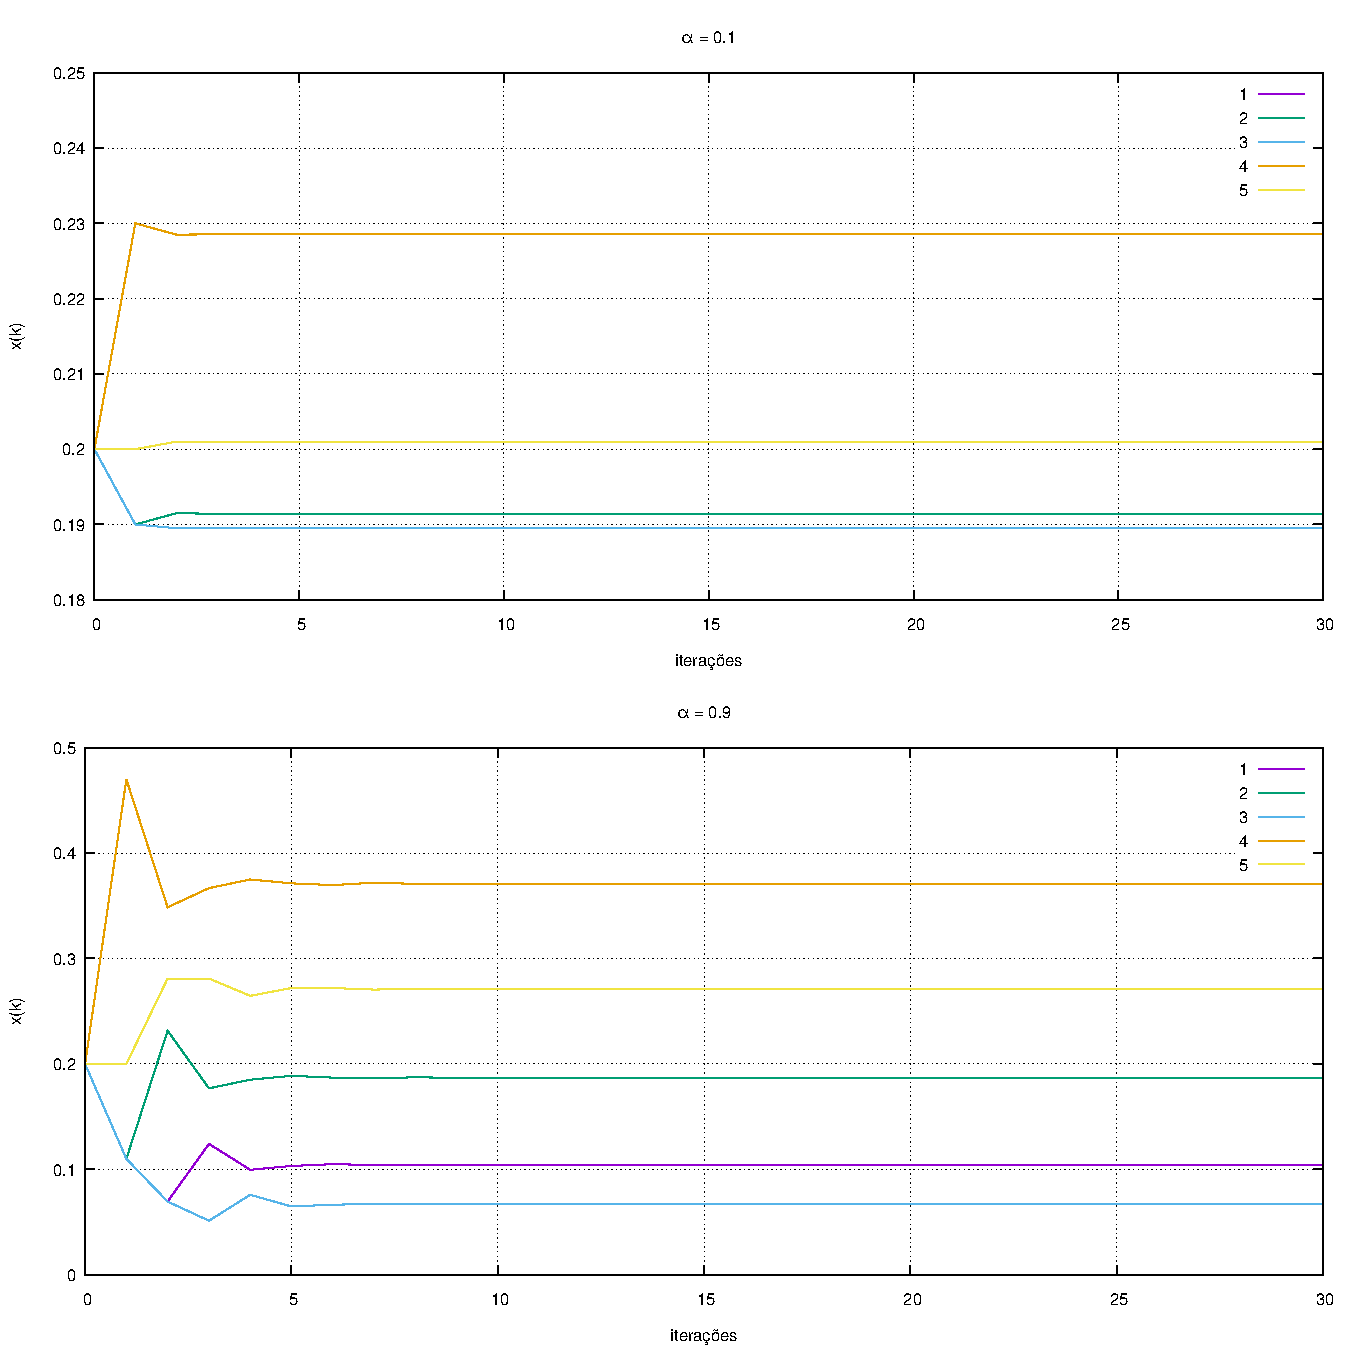
\includegraphics[width=\textwidth]{"../src/plot/pagerank.pdf"}
	\end{fig}

	\quest{Similaridade entre vértices}%% 7

	\begin{fig}[Grafo de \textit{Barbell} $\mathcal{B}_{4, 2}$]
		\begin{tikzpicture}
	\ttfamily
	\def\tks{2}
	\begin{pgfonlayer}{nodelayer}
		\node [style=plains] (0) at (-2.5 * \tks, 1 * \tks) {a};
		\node [style=plains] (1) at (-1.5 * \tks, 1 * \tks) {c};
		\node [style=plains] (2) at (-2.5 * \tks, 0 * \tks) {ξ};
		\node [style=plains] (3) at (-1.5 * \tks, 0 * \tks) {b};
		\node [style=plains] (4) at (-0.5 * \tks, 1 * \tks) {d};
		\node [style=plains] (6) at (0.5 * \tks, 1 * \tks) {e};
		\node [style=plains] (7) at (1.5 * \tks, 1 * \tks) {f};
		\node [style=plains] (8) at (2.5 * \tks, 1 * \tks) {g};
		\node [style=plains] (9) at (1.5 * \tks, 0 * \tks) {*};
		\node [style=plains] (10) at (2.5 * \tks, 0 * \tks) {*};
	\end{pgfonlayer}
	\begin{pgfonlayer}{edgelayer}
		\draw (0) to (2);
		\draw (0) to (3);
		\draw (3) to (1);
		\draw (1) to (2);
		\draw (2) to (3);
		\draw (0) to (1);
		\draw (1) to (4);
		\draw (6) to (7);
		\draw (7) to (9);
		\draw (7) to (8);
		\draw (7) to (10);
		\draw (8) to (10);
		\draw (9) to (10);
		\draw (8) to (9);
		\draw (4) to (6);
	\end{pgfonlayer}
\end{tikzpicture}

	\end{fig}

	\subquest{}%%1
	Recapitulando as definições da similaridade de \textit{Jaccard} $\mathcal{J}(i, j)$ e da similaridade do Cosseno $\mathcal{C}(i, j)$ dizemos que
		$$\mathcal{J}(i, j) = \frac{\norm[0]{\adj i \cap \adj j}}{\norm[0]{\adj i \cup \adj j}} ~\text{ e }~ \mathcal{C}(i, j) = \frac{\inner{\vet{A}_i}{\vet{A}_j}}{\norm{\vet{A}_i} \cdot \norm{\vet{A}_j}} = \frac{\norm[0]{\adj i \cap \adj j}}{\sqrt{\norm[0]{\adj i} \cdot \norm[0]{\adj j}}}$$
	onde $\adj \xi$ denota o conjunto dos vértices na vizinhança de $\xi$ e $\vet{A}_\xi$ é a linha correspondente na matriz de adjacências.\par

	Organizando os resultados em uma tabela:

	\begin{fig}
		\begin{tabular}{|c|c|c|c|c|r|r|}
		\hline
		$i, j$ & $\adj i$ & $\adj$ j & $\adj i \cap \adj j$ & $\adj i \cup \adj j$ & $\mathcal{J}(i, j)$ & $\mathcal{C}(i, j)$\\
		\hline
		$a, b$ & \set{b, c, \xi} & \set{a, c, \xi} & \set{c, \xi} & \set{a, b, c, \xi} & .50 & .66 \\
		\hline
		$b, c$ & \set{a, c, \xi} & \set{a, b, d, \xi} & \set{a, \xi} & \set{a, b, c, d, \xi} & .40 & .58\\
		\hline
		$c, d$ & \set{a, b, d, \xi} & \set{c, e} & \set{} & \set{a, b, c, d, e, \xi} & 0 & 0 \\
		\hline
		$d, e$ & \set{c, e} & \set{d, f} & \set{} & \set{c, d, e, f} & 0 & 0 \\
		\hline
		\end{tabular}
	\end{fig}

	\subquest{}%%2
	Não, muito pelo contrário. Como ambas possuem a interseção das vizinhanças no numerador, vértices cujas conexões são idênticas a menos de isomorfismo não serão contemplados por estas duas métricas. Do ponto de vista da \textit{identidade estrutural}, poderíamos afirmar que os vértices $d$ e $e$ são estruturalmente idênticos. Se alguém removesse as etiquetas da Figura \ref{fig:7.1} e chacoalhasse o grafo um pouco, já seria impossível afirmar com certeza quais vértices estavam marcados por $d$ e $e$. No entanto, em ambas as métricas este par de vértices foi tratato como plenamente dissemelhante.

	\subquest{}%%3
	O grafo de \textit{Barbell} foi colorido na figura abaixo de modo que dois vértices possam ter suas identidades trocadas e ainda pertencer a um automorfismo $\sigma$ caso tenham sido coloridos com a mesma cor.

	\begin{fig}[Um mapa para o Automorfismo]
		\begin{tikzpicture}
	\ttfamily
	\def\tks{2}
	\begin{pgfonlayer}{nodelayer}
		\node [style=plains, fill=red!40] (0) at (-2.5 * \tks, 1 * \tks) {a};
		\node [style=plains, fill=orange!40] (1) at (-1.5 * \tks, 1 * \tks) {c};
		\node [style=plains, fill=red!40] (2) at (-2.5 * \tks, 0 * \tks) {ξ};
		\node [style=plains, fill=red!40] (3) at (-1.5 * \tks, 0 * \tks) {b};
		\node [style=plains, fill=yellow!40] (4) at (-0.5 * \tks, 1 * \tks) {d};
		\node [style=plains, fill=yellow!40] (6) at (0.5 * \tks, 1 * \tks) {e};
		\node [style=plains, fill=orange!40] (7) at (1.5 * \tks, 1 * \tks) {f};
		\node [style=plains, fill=red!40] (8) at (2.5 * \tks, 1 * \tks) {g};
		\node [style=plains, fill=red!40] (9) at (1.5 * \tks, 0 * \tks) {*};
		\node [style=plains, fill=red!40] (10) at (2.5 * \tks, 0 * \tks) {*};
	\end{pgfonlayer}
	\begin{pgfonlayer}{edgelayer}
		\draw (0) to (2);
		\draw (0) to (3);
		\draw (3) to (1);
		\draw (1) to (2);
		\draw (2) to (3);
		\draw (0) to (1);
		\draw (1) to (4);
		\draw (6) to (7);
		\draw (7) to (9);
		\draw (7) to (8);
		\draw (7) to (10);
		\draw (8) to (10);
		\draw (9) to (10);
		\draw (8) to (9);
		\draw (4) to (6);
	\end{pgfonlayer}
\end{tikzpicture}

	\end{fig}

\end{document}